% mnras_template.tex
%
% LaTeX template for creating an MNRAS paper
%
% v3.0 released 14 May 2015
% (version numbers match those of mnras.cls)
%
% Copyright (C) Royal Astronomical Society 2015
% Authors:
% Keith T. Smith (Royal Astronomical Society)

% Change log
%
% v3.0 May 2015
%    Renamed to match the new package name
%    Version number matches mnras.cls
%    A few minor tweaks to wording
% v1.0 September 2013
%    Beta testing only - never publicly released
%    First version: a simple (ish) template for creating an MNRAS paper

%%%%%%%%%%%%%%%%%%%%%%%%%%%%%%%%%%%%%%%%%%%%%%%%%%
% Basic setup. Most papers should leave these options alone.
\documentclass[a4paper,fleqn,usenatbib]{mnras}

% MNRAS is set in Times font. If you don't have this installed (most LaTeX
% installations will be fine) or prefer the old Computer Modern fonts, comment
% out the following line
\usepackage{newtxtext,newtxmath,amsmath}
% Depending on your LaTeX fonts installation, you might get better results with one of these:
%\usepackage{mathptmx}
%\usepackage{txfonts}

% Use vector fonts, so it zooms properly in on-screen viewing software
% Don't change these lines unless you know what you are doing
\usepackage[T1]{fontenc}
\usepackage{ae,aecompl}
\usepackage{amsmath}
\usepackage{pbox}

%%%%% AUTHORS - PLACE YOUR OWN PACKAGES HERE %%%%%

% Only include extra packages if you really need them. Common packages are:
\usepackage{graphicx}	% Including figure files
\usepackage{amsmath}	% Advanced maths commands
\usepackage{amssymb}	% Extra maths symbols
\usepackage{gensymb}
\usepackage{subfig}

\usepackage{todonotes}

%%%%%%%%%%%%%%%%%%%%%%%%%%%%%%%%%%%%%%%%%%%%%%%%%%

%%%%% AUTHORS - PLACE YOUR OWN COMMANDS HERE %%%%%

% Please keep new commands to a minimum, and use \newcommand not \def to avoid
% overwriting existing commands. Example:
%\newcommand{\pcm}{\,cm$^{-2}$}	% per cm-squared

%%%%%%%%%%%%%%%%%%%%%%%%%%%%%%%%%%%%%%%%%%%%%%%%%%

%%%%%%%%%%%%%%%%%%% TITLE PAGE %%%%%%%%%%%%%%%%%%%

% Title of the paper, and the short title which is used in the headers.
% Keep the title short and informative.
\title[The luminosity dependence of disc winds in XRBs]{The luminosity dependence of thermally-driven disc winds in X-ray binaries}
%\title[Increasing luminosity]{Radiation-hydrodynamic simulations of thermally-driven disc winds in X-ray binaries: Increasing
%luminosity reveals a constant wind efficiency}

% The list of authors, and the short list which is used in the headers.
% If you need two or more lines of authors, add an extra line using \newauthor
\author[N. Higginbottom et. al]
{Nick Higginbottom,$^{1}$\thanks{E-mail: nick\_higginbottom@fastmail.fm}
Christian Knigge$^{1}$, Knox S. Long$^{2,3}$, 
James H. Matthews$^{4}$ \newauthor{and
Edward J. Parkinson$^{1}$.}
\\
% List of institutions
$^{1}$School of Physics and Astronomy, University of Southampton, Highfield, Southampton, SO17 1BJ, UK\\
$^{2}$Space Telescope Science Institute, 3700 San Martin Drive, Baltimore, MD, 21218, USA\\
$^{3}$Eureka Scientific Inc., 2542 Delmar Avenue, Suite 100, Oakland, CA, 94602-3017, USA\\
$^{4}$University of Oxford, Astrophysics, Keble Road, Oxford OX1 3RH, UK\\
$^{5}$School of Mathematics and Physics, Queen's University Belfast, University Road, Belfast 
BT7 1NN, UK\\
}

% These dates will be filled out by the publisher
\date{Accepted XXX. Received YYY; in original form ZZZ}

% Enter the current year, for the copyright statements etc.
\pubyear{2018}

% Don't change these lines
\hypersetup{draft}
\begin{document}
\label{firstpage}
\pagerange{\pageref{firstpage}--\pageref{lastpage}}
\maketitle

% Abstract of the paper
\begin{abstract}

  We have carried out radiation-hydrodynamic simulations of
  thermally-driven accretion disc winds in X-ray binaries. Our main
  goal is to study the luminosity dependence of these outflows. The 
  simulations span the range 
  $0.04 \leq L_{acc}/L_{Edd} \leq 1.0$ and therefore cover most of the parameter
  space in which disc winds have been observed. We
  find that (i) the wind {\em
  efficiency} always remains approximately
  constant, $\dot_{M}_{wind}/\dot{M}_{acc} \simeq
  2$; (ii) the wind velocity 
  increases with luminosity, roughly as $v \propto L_{acc}^{1/4}$;
  (iii) the large-scale wind geometry is quasi-spherical, but 
  observable absorption features are preferentially produced along
  high-column equatorial sightlines; (iv) with increasing luminosity,
  detectable high-ionization absorption features are produced at lower 
  inclinations. In order to illustrate the observational signatures of such
  outflows, we also present synthetic Fe \textsc{xxv}
  and Fe \textsc{xxvi} absorption line profiles for our simulated disc winds.


\end{abstract}

% Select between one and six entries from the list of approved keywords.
% Don't make up new ones.
\begin{keywords}
Accretion discs -- hydrodynamics -- methods:numerical -- stars:winds -- X-rays:binaries
\end{keywords}

%%%%%%%%%%%%%%%%%%%%%%%%%%%%%%%%%%%%%%%%%%%%%%%%%%

%%%%%%%%%%%%%%%%% BODY OF PAPER %%%%%%%%%%%%%%%%%%

\section{Introduction}
Signatures of outflowing gas have been observed in essentially all
types of disk-accreting astrophysical systems, from protostars,
cataclysmic variables and X-ray binaries to Seyfert Galaxies and
Quasars. Highly collimated fast jets are often the most spectacular
type of outflow from these systems. However, less collimated, slower
and more higly mass-loaded disk winds are at least as common and can 
actually have a more significant impact, both on the environments of
these systems and on the accretion flow itself. 
 
X-ray binaries (XRBs) are systems in which secondary star transfers mass to a compact primary (either a black hole or a neutron star)
via an accretion disk. They are excellent laboratories in which to
study the accretion physics, with lessons learned from XRBs often finding application also in AGN and other systems) \citep{2003MNRAS.345L..19M,2004A&A...414..895F,2006MNRAS.372.1366K,
2001MNRAS.323L..26U,
2015SciA....1E0686S,
2014MNRAS.438.1233S,
2013MNRAS.431.2535S,
2012MNRAS.421.2854S,	
2008Sci...320.1318K,
2018MNRAS.481.2140A,
2015MNRAS.448.2430V}.
In particular, XRBs exhibit dramatic changes in their spectra and luminosity over timescales on the order of days
\cite[e.g.][]{1999ApJ...520..776S,2004ApJ...610..378P}, which can be
linked to changes in the nature of the accretion flow
\cite[e.g.][]{1995PASP..107.1207N,2012Sci...337..540F}. Disk winds are 
seen when systems are in the ``high-soft'' state, during which the accretion disk is thought to extend all the way to the 
central compact object \cite[][although see \citealt{2016ApJ...830L...5H}]{2012MNRAS.422L..11P}. Disc wind signatures are not generally
observed in the ``low-hard'' state, during which the inner disk appears to be truncated, and the X-ray emission is dominated by a
Comptonised corona. This suggests that disc winds might play a role in
regulating -- and perhaps triggering -- state changes in XRBs. In
fact, for sufficiently high mass-loss rates, disc winds are {\em
  expected} to destabilize a steady accretion flow through the 
disc \citep{1986ApJ...306...90S}.

We are therefore interested in developing a theoretical model for
these disk winds, with an eye to 
predicting their mass-loss rates and hence testing the possibility
that they are indeed responsible for state changes. Unfortunately, even the
basic driving mechanism for these disk winds remains a topic of much
debate and active research. However, broadly speaking, there are three main contenders --
radiation driving, thermal driving, and magneto-centric driving. 

The first mechanism, radiation driving, involves the transfer of
momentum from the radiation field to outflowing matter. This transfer
can take place via Compton scattering or via the scattering of (mainly
UV) photons by bound-bound transitions. If the ionisation state of the gas is 
favourable, the latter ``line-driving'' mechanism can
produce a radiation pressure more than 1000$\times$ higher than that
due to Compton scattering \citep{1975ApJ...195..157C,
1995ApJ...454..410G}. In X-ray binaries, 
the observed absorption lines suggest that the outflow is highly ionised \citep[e.g.][]{2009ApJ...701..865K,
2018ApJ...861...26A}, with an ionization parameter $\xi \geq 3$
\citep{2016AN....337..368D}. In such an environment, line-driving is
unlikely to be important. However, the luminosity of some XRBs can
approach or even exceed the Eddington limit, so radiation driving via
Compton scattering alone may be sufficient to drive -- or at least
affect -- the outflow.

The second mechanism, thermal driving, produces outflows whenever gas
is heated to a temperature at which the thermal velocity exceeds
the local escape velocity. In this situation, mass-loss is
inevitable. This mechanism is particularly attractive in 
X-ray binaries, where the high-energy radiation emitted close to the
accretor can irradiate the outer disk, producing a high-temperature
surface layer in which thermal speeds can exceed the escape velocity. As a rule of thumb, thermal winds might be expected
to arise at or just inside the Compton Radius ($\rm{R_{IC}}$) - the radius at which gas at the Compton temperature ($T_C$ - 
the temperature at which the Compton heating and cooling rates balance)
for a given source SED corresponds to a thermal velocity in excess of
the escape velocity \citep{1983ApJ...271...70B}. More specifically,
$R_{IC}$ is given by 
\begin{equation}
R_{IC}=\frac{GM_{BH}\mu m_H}{k_BT_C},
\end{equation}
where $M_{BH}$ is the mass of the central object, $\mu$ is the 
mean molecular mass (which we set to 0.6), and the other symbols have the usual meaning. 
For our SED, $T_C=1.4\times10^7$~K, so $R_{IC}=4.82\times10^{11}$ - about $4.6\times10^5$ gravitational
radii.


%%%%%%%%%%%%%%%%%%%%%%%%%%%%%%%%%%%%%%%%%%%%%%

The third proposed mechanism is that of magneto-centrifugal driving. 
Observations of the disk-wind in GRO J1655-40 in a peculiar `hypersoft' state suggested that the wind in that
case arose well inside $\rm{R_{IC}}$. In such a case the existence of a thermal wind is harder to justify 
and magneto-centrifugal driving has been suggested as an alternative driving mechanism
\citep[but also see \citealt{2006ApJ...652L.117N,2015MNRAS.451..475U,2016ApJ...823..159S}]
{1992ApJS...80..753S,2006Natur.441..953M,2008ApJ...680.1359M,2009ApJ...701..865K}. Since
magnetic fields are essential in the evolution of accretion disks, it is not unreasonable to expect such winds to 
exist. In such a wind, ionized material is loaded onto magnetic field lines leaving the accretion disk, and via a process
of angular momentum conservation, the material is accelerated as it moves out along the field lines, like beads
on a wire.

Most likely, all three mechanisms are at play, perhaps changing their importance depending on the
geometry and accretion state of the source in question. Of the three mechanisms, thermal driving is 
particularly interesting in X-ray binaries because it is almost certain to 
operate on some level wherever there is strongly heated gas and a disk of sufficient radial extent that hot gas 
can escape. Indeed, this mechanism might not only be important in X-ray binaries but also in protoplanetary systems \cite[e.g.][]{2012MNRAS.422.1880O} and AGN \cite[e.g.][]{2018MNRAS.476.4395B}.

The existence of thermally driven outflows from accretion disks has been postulated since such disks were themselves
first considered \citep{1973A&A....24..337S}. More detailed theoretical treatment of thermal winds \citep{1983ApJ...271...70B} suggested that the mass-loss could be sufficient to destabilise the disk \citep{1986ApJ...306...90S}.
As computer power improved, more detailed hydrodynamic simulations  \citep{1996ApJ...461..767W,2006ApJ...652L.117N,2010ApJ...719..515L,2015ApJ...807..107H} have provided support for the earlier predications of large mass-loss rates and also showed that thermal winds could provide a source of observed blue shifted absorption lines.

Although very large mass-loss rates are possible through thermal winds, the actual rate is very 
dependant on the details
 of the heating/cooling rates  \citep{2017ApJ...836...42H}. These 
in turn depend critically on the source SED \citep{2017MNRAS.467.4161D} and any attenuation effect between the source and the wind
launching region. \citet[hereafter H18]{2018MNRAS.479.3651H} presented a radiation-hydrodynamic simulation which 
took account
of this attenuation by coupling the radiative transfer code  \textsc{python} to the hydrodynamics code \textsc{zeus} and 
found that there was still an appreciable outflow, with about two and a half times as much material outflowing as was required
to produced the observed luminosity through accretion. In addition, reasonable agreement was found between 
Lyman $\alpha$ lines of helium and hydrogen like iron generated from the simulation and those seen in \emph{Chandra} 
observations of the LMXB GRO J1655-40 in the soft-intermediate state. 

That simulation was for a luminosity of 4 per cent of the Eddington luminosity  ($\rm{L_{Edd}}$) for a 7 solar mass 
central black hole but disk winds have been observed in systems with luminosities up to or even slightly exceeding 
$\rm{L_{Edd}}$ \citep[][herafter P12]{2012MNRAS.422L..11P}.  Observations
suggest that the wind efficiency (mass loss rate divided by mass accretion rate) may increase with luminosity, 
(P12, although this relationship is driven by observations of a single exceptional source) whilst recent theoretical work 
suggests that the wind efficiency tends to a constant value \citep[][hereafter D18]{2018MNRAS.473..838D}.

Here, we extend our radiation hydrodynamic simulations to higher 
luminosities in order to investigate the effect on mass loss rate and velocity in the resulting outflows. 
As discussed in Section \ref{section:method}, we  use the same technique as H18 with slight modifications for varying the luminosity.
We then present our results in Section \ref{section:results} before making comparisons to observations in Section \ref{section:discussion}.


 

\section{Method }
\label{section:method}

As in H18, we use an operator splitting radiation-hydrodynamic method to treat the propagation of radiation
from a central source through the wind. We use the hydrodynamic code {\sc zeus} 
\citep[][extended by \citealt{2000ApJ...543..686P}]{1992ApJS...80..753S}, coupled to our own ionization and
 radiative transfer code {\sc python} \citep[][extended by \citealt{,2013MNRAS.436.1390H} and 
 \citealt{2015MNRAS.450.3331M}]{2002ApJ...579..725L}. 

Since thermal winds are expected to arise at or just inside $\rm{R_{IC}}$, which is independent of the source 
luminosity, we leave the simulation geometry unchanged
from H18, and simply increase the luminosity. We use the same logarithmic grid, the parameters of which are given in the upper
part of Table \ref{table:wind_param}. The mid-plane of the simulation space is set up with a constant 
density boundary condition, forming a mass reservoir for any resulting outflow. The value of this constant density
is important, since the wind is generated when the ionization parameter reaches the critical value $\xi_{cool,max}$ which
represents the maximum ionization parameter for gas on the `cool branch' of the thermal stability curve. Gas with
$\xi<\xi_{cool,max}$ has a stable temperature of a few tens of thousands K where line/recombination cooling 
balances photoionization heating. 

At higher ionization parameters, the gas becomes thermally unstable and heats up rapidly. 
This heating causes expansion and
a wind is driven. We refer to the part of the wind where this acceleration occurs as the acceleration zone.
In the optically thin limit one can set the mid-plane density so that gas at the mid-plane has
exactly the right ionization parameter. This means that the acceleration zone occurs in the cells directly 
above the mid-plane, avoiding including static material in the simulation, and thus maximizing the resolution in the acceleration zone.

In the simulations presented here attenuation of the radiation is treated fully and it is therefore not possible to 
compute the ionization parameter for a given cell a-priori since it depends not only on the local density  
but also on the density of the developing wind along the 
sightline back to the source. 
We therefore set the mid-plane density using the optically thin ionisation parameter,
finding that a small wedge of static material does form due to optical depth effects. However the extent of this does not significantly
affect the resolution in the acceleration zone. The mid-plane densities we have used are given in Table 
\ref{table:wind_param}. They are proportional to the source luminosity,  thereby preserving the same
ionization parameter (in the optically thin approximation).

All other aspects of the simulation are identical to that described by H18, including a truncation of the 
mid-plane density boundary condition at $\rm{R=2 R_{IC}}$.

\begin{table}
\begin{tabular}{p{3.0cm}p{0.8cm}p{0.8cm}p{0.8cm}p{0.8cm}}
\hline 
Luminosity ($\rm{L_{edd}}$) & 0.04 & 0.1 & 0.3 & 0.6 \\ 
\hline 
\hline Physical Parameters & & & \\ \hline
$\rm{M_{BH}~(M_{\odot})}$  & 7 & 7 & 7 &7\\
$\rm{T_x~(10^7~}$K)  & 5.6 & 5.6 & 5.6  & 5.6\\
$\rm{L_x~(10^{37}}~\rm{ergs~s^{-1}})$&  3.3& 8.25 &  24.75 &49.5\\
$\dot{\rm{M}}_{\rm{acc}}~(10^{17}~\rm{ergs~s^{-1}})$&  4.42 & 11.1 &  33.2 &66.3\\
$\rm{\log(\xi_{cold,max})}$&   1.35 & 1.35 & 1.35 & 1.35 \\
$\rm{T_{eq}(\xi_{cold,max})~(10^3~K)}$ &  50.7 &  50.7 & 50.7 & 50.7 \\
$\rm{\rho_0~(10^{-12}~g~cm^{-3})}$  & 16.0 & 40 & 120 & 240 \\
$\rm{R_{IC}~(10^{11}~cm)}$  & 4.82 & 4.82 & 4.82 & 4.82 \\
\hline
\multicolumn{4}{l}{Derived wind properties}\\
\hline 
\multicolumn{4}{l}{$\rm{V_r~(\rho>1\times10^{12})}$}  \\
$\rm{max,blueshifted~({km~s^{-1}})}$ &  50 & 68 & 256  & 150  \\
$\rm{V_r(max,\theta>60\degree~({km~s^{-1}})}$ &  259   & 374 & 533    & 642 \\
$\rm{N_H~(70\degree)~(10^{22}}~\rm{cm^{-2})}$ & 2.0 & 4.0 &  8.3 & 13 \\
$\rm{N_H~(80\degree)~(10^{22}}~\rm{cm^{-2})}$  & 4.2 & 8.4 & 16 & 25 \\
${\dot{\rm{M}}_{\rm{wind,outer}}~(10^{18}~g~s^{-1}})$  &  1.1 & 2.7 &  6.7  & 12.7 \\
${\dot{\rm{M}}_{\rm{wind,outer}}~(\dot{\rm{M}}_{\rm{acc}})}$  & 2.5 & 2.4 & 2.0 & 1.9  \\
${0.5\dot{\rm{M}}\rm{V_r^2}~(10^{32}}~\rm{erg~s^{-1}})$  &  4.2 & 21.3 &   109 & 310  \\


\hline
\end{tabular}
\caption{Parameters adopted in the simulations, along with key properties of the resulting outflows.}
\label{table:wind_param}
\end{table}



\section{Results}
\label{section:results}

\begin{figure*}
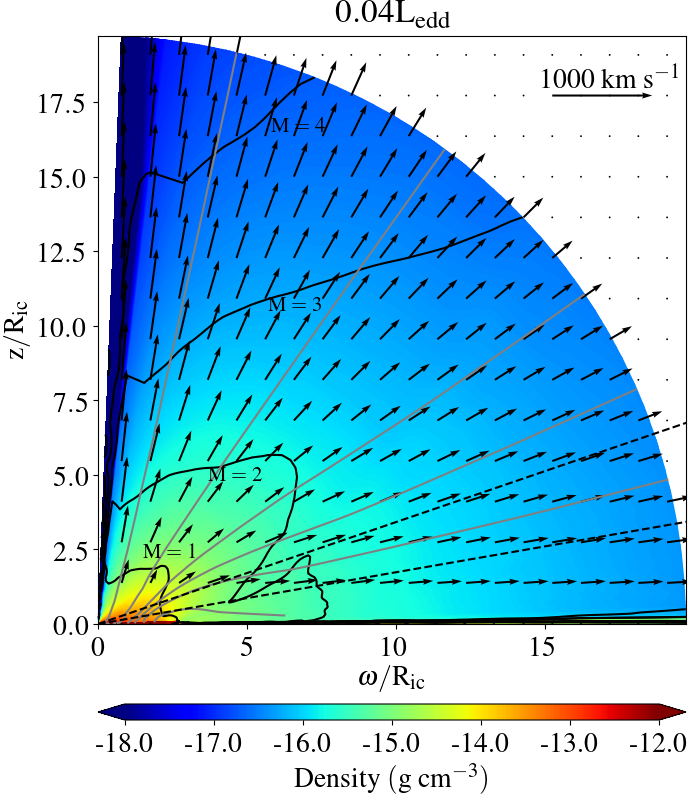
\includegraphics[width=\columnwidth]{figures/fig3a_density.png}
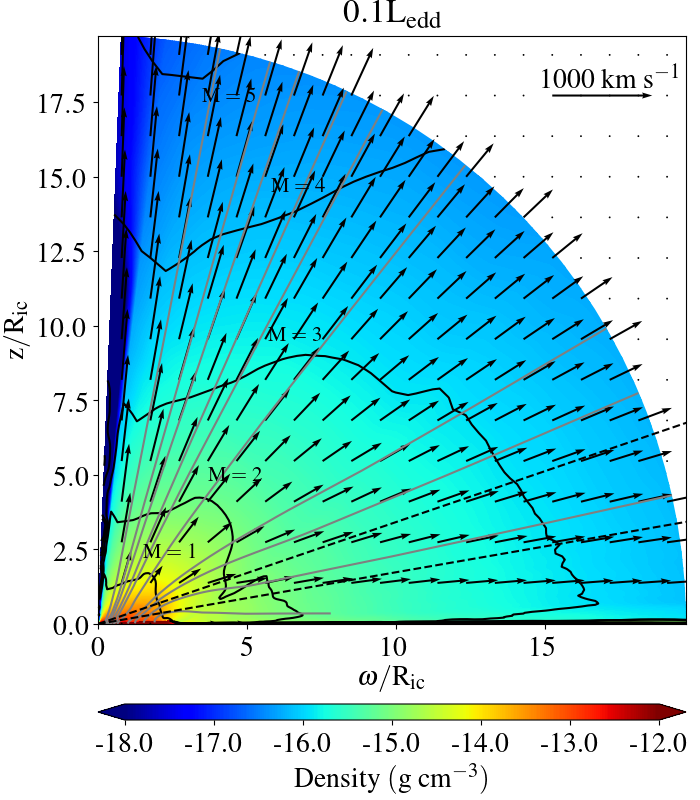
\includegraphics[width=\columnwidth]{figures/fig3b_density.png}
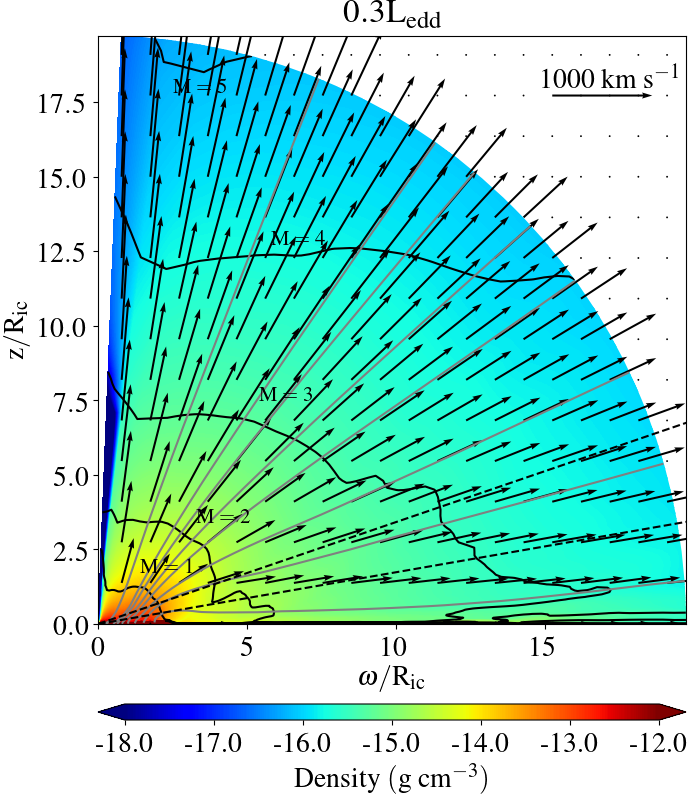
\includegraphics[width=\columnwidth]{figures/fig3c_density.png}
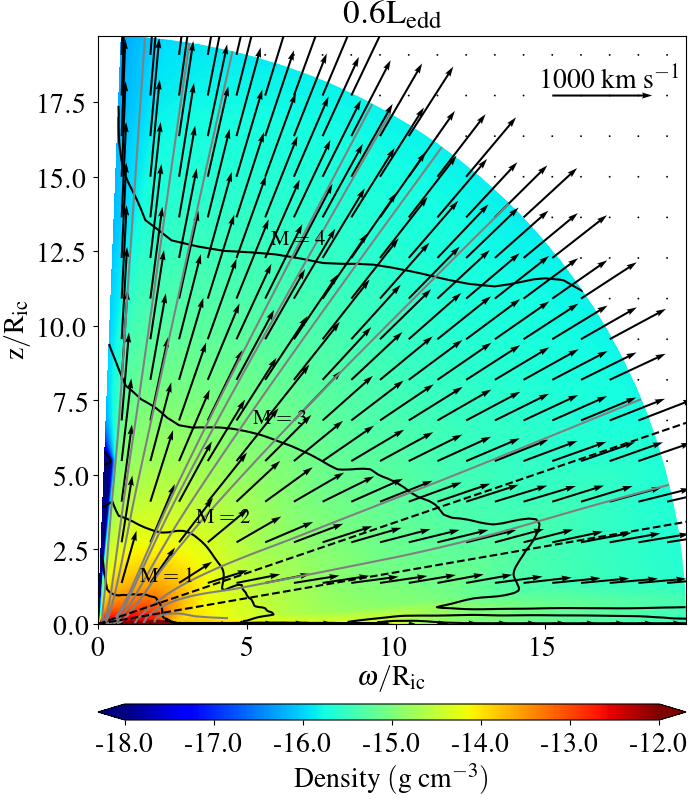
\includegraphics[width=\columnwidth]{figures/fig3d_density.png}
\caption{The density (colours) and velocity structure (arrows) of the stable final states for 
four different luminosities. Grey lines show streamlines, and the black line shows the location of the Mach surfaces. The two dotted
lines show the location of the $70\degree$ and $80\degree$ sightlines.}
\label{figure:wind_small_image}
\end{figure*}

We have computed disk-wind models for central source luminosity 
$\rm{L=0.1~L_{Edd}-1.0~L_{Edd}}$ in steps of $\rm{0.1~L_{Edd}}$. In each case, the simulations reach stable states, 
with static disk-like wedges forming at the base of the simulation as seen in H18. The reason for this
structure is attenuation of the radiation through the disk. So, if a cell at a given angle has just the right
conditions to launch a wind, the cell behind it will be slightly obscured and so on until at a certain radius
the radiation is attenuated to the point at which a wind is launched from the next theta cell 'up'. This gives
rise to a thin, slightly convex disk structure. 

Because we increase the mid-plane density in proportion to the luminosity in order to try and maintain 
a fixed ionization parameter at the base of the wind, the shape of the disk structure slightly changes as
the luminosity increases. In all cases, at the inner radial edge, the disk/wind interface occurs at 
around 89\degree~from the z-axis (i.e. 1\degree~ above the mid-plane). For the original $\rm{0.04L_{Edd}}$ 
simulation, the angle at which the interface occurs decreases to about 88\degree~ at the outer edge, whereas for 
the $\rm{L_{Edd}}$ simulation, the interface is about a degree further from the
midplane at 87\degree.

Density contour plots for some of the resulting outflows are shown in Figure \ref{figure:wind_small_image}.
We concentrate here, and in the rest of the results/discussion sections, on the calculations using luminosities
up to 60 per cent of $L_{Edd}$. This is because we do not treat radiation driving, a process
that would become increasingly important as the luminosity approaches $L_{Edd}$.
It is clear from these images that the velocity of the outflows increases with luminosity, as does the 
density in the wind. Some useful parameters showing this are given in the lower part of Table \ref{table:wind_param}.
As one would expect, the mass-loss rate through the outer boundary, which is essentially a function of these 
two parameters also increases with luminosity. We will discuss this further in the next section. The velocity field 
becomes somewhat more `spherical' as the luminosity increase, however the nature of the wind is still equatorial.
This is because the density distribution is still concentrated towards the mid-plane. Having said that, since the overall
density increases, a given column density is reached further from the midplane as the density increases.
\textcolor{red}{possibility of numbers here to discuss the angle at which a given $N_H$ or EW 
in a given line is reached}.




\section{Discussion}
\label{section:discussion}


\subsection{Mass-loss rates}

The mass-loss rates ($\dot{\rm{M}}_{\rm{wind,outer}}$) listed in Table \ref{table:wind_param}  
increase as the luminosity of the central source increases. However when we  compare these values to the implied
accretion rate ($\dot{\rm{M}}_{\rm{acc}}$) we find that $\dot{\rm{M}}_{\rm{wind,outer}}\simeq2\dot{\rm{M}}_{\rm{acc}}$
for all cases.
This constant `wind efficiency' is similar to that found in the analysis carried out by \cite{2018MNRAS.473..838D}
who found that for a disk of our size ($R_{out}=2R_{IC}$) and a Compton temperature
very close to ours the wind efficiency peaked at just over two for a luminosity close to our lowest luminosity.
They then see the efficiency decrease slowly with increasing luminosity, 
always remaining above one. Our wind efficiencies are slightly larger than theirs, which is interesting since
we neglect any radiation driving effects, which they include via an approximate correction. 

The wind efficiency for a range of observed XRB winds is given by \cite{2012MNRAS.422L..11P}.
It is instructive to compare our results with these observations. Figure \ref{figure:mdot_vs_lum} shows 
this comparison, with the black symbols referring to the observations and the red stars showing the
results of these simulations. 

\begin{figure}
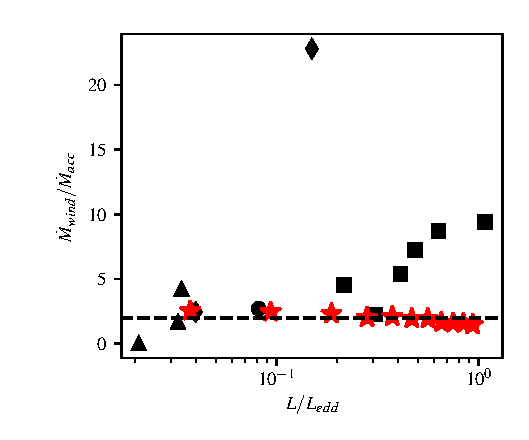
\includegraphics[width=\columnwidth]{figures/ponti.eps}
\caption{$\rm{\dot{M}_{wind}/\dot{M}_{acc}}$ vs. luminosity based upon figure 5 in \citet{2012MNRAS.422L..11P}. 
Black symbols are empirical values obtained from {\em Chandra} HETG data for several LMXBs. 
The symbols refer to the specific object each measurement refers to 
(triangles = H1743-322; circles = 4U~1640-47; squares = GRS~1915+105; diamonds = GRO~J1655-40). 
The red stars represent the results of the simulations presented here, and the dotted line
is at $\rm{\dot{M}_{wind}/\dot{M}_{acc}}$=2.0.}
\label{figure:mdot_vs_lum}
\end{figure}

At first sight, our prediction of a constant wind efficiency does not appear to
agree with the observations, which appear to suggest an increase of wind efficiency with
luminosity. However, the increase in wind efficiency with luminosity is largely driven 
by observations of just one source - GRS 1915 +105.  This is an exceptional source, which has been 
accreting close to the Eddington limit since its discovery in 1992  never
entering quiescence \citep{1994ApJS...92..469C,2017MNRAS.468.4748C}. 
It also exhibits unusual SEDs, not corresponding to the normal high/soft,
low/hard spectral states \citep{2016ApJ...833..165Z}. Finally, with an orbital period of 34 days 
\citep{2014SSRv..183..223C} this is by far the largest system - and could perhaps host a signficantly
larger accretion disk than we include in our model. This complex source requires more detailed
analysis and modelling which is beyond the scope of this study. Setting aside the observations of this
source, the rest show reasonable consistency with wind efficiency around two over a significant 
range of luminosities, as seen in the simulations.

\subsection{Comparison to B83 calculations}
\label{Section:B83}
A useful way of categorising different classes of thermally driven winds was introduced 
by \cite[hereafter B83]{1983ApJ...271...70B}, and further developed by \cite[hereafter W96]{1996ApJ...461..767W}. The
diagram from B83 is reproduced in Figure  \ref{figure:regions}. The vertical axis is the luminosity of the central
source in units of the `critical luminosity' defined as
\begin{equation}
L_{crit}=0.03T_{C,8}^{-1/2}L_{Edd}
\label{L_crit}
\end{equation}
where $T_{C,8}$ is the Compton temperature in units of $10^8$~K,
whilst the horizontal axis is the radius on the disk where streamline arises normalised to the Compton radius. 

\begin{figure}
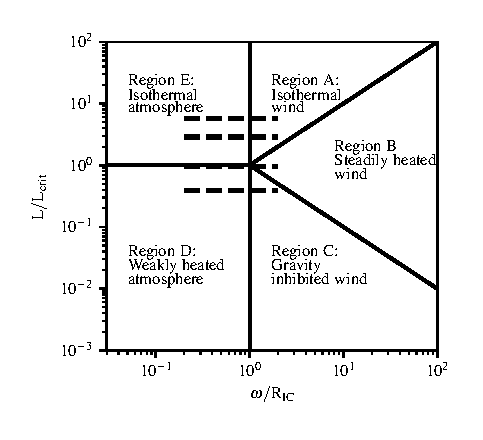
\includegraphics[width=\columnwidth]{figures/fig7.eps}
\caption{Regions of different wind solutions after \protect\cite{1983ApJ...271...70B}. The horizontal dashed 
lines represent the luminosity and disk extent of the simulations in H18
(lowest line) and those presented here}
\label{figure:regions}
\end{figure}

The different regions designate different types of outflow or static atmosphere, and are a consequence of
how quickly the plasma is heated. The regions in the lower half of the Figure heat slowly 
whilst regions in the upper half heat rapidly to the Compton temperature. The regions on the
right hand side are where gas at the Compton temperature would be expected to escape, whilst on the 
left hand side the gas is gravitationally bound and so forms an atmosphere rather than a wind. 
In regions B and C, the gas flows outwards too quickly to be heated to the Compton temperature. In region
B the gas temperature still exceeds the temperature needed to escape at the radius at which it is launched, 
whereas in region C it does not even reach that temperature and so the gas remains gravitationally
bound.

B83 found that there was not a clear dividing line between bound and unbound solutions 
at $\rm{\omega=R_{IC}}$. W96 found that a more reasonable location for this cutoff was 
$\rm{\omega=0.1 R_{IC}}$.
Our 4 per cent simulation represents about $\rm{0.5 L_{crit}}$ and is shown on Figure \ref{figure:regions} as the lowest 
horizontal dashed line. The 10 per cent simulation (next horizontal line up) has a luminosity just below $\rm{L_{crit}}$ 
and
the two higher luminosity cases are above $\rm{L_{crit}}$. We would therefore expect to see a clear difference between the lowest luminosity case and the two higher cases with gas impulsively heated to the Compton
temperature in the latter. However, although the outflowing gas gets hotter as the luminosity increases in no
case does it approach $\rm{T_{IC}}$. In fact we see that, as the gas expands and accelerates
away, adiabatic cooling increases quickly and balances Compton heating and X-ray heating in much of the wind. The gas heats up initially, reaching a peak temperature at a distance of about $R_{IC}$ along the streamline of between
about $1\times10^6$~K for the low luminosity case and $6\times10^6$~K for $L=L_{Edd}$. The temperature then starts dropping. 

The Bernoulli parameter is given by $Be\equiv\bold{v}^2+\gamma P/(\gamma-1)\rho-GM_{bh}/r$, where the first
term is the kinetic energy of the gas with velocity $\bold{v}$, the second term is the gas enthalpy and the third
term is the gravitational potential. $Be$ is negative at the streamline roots; the gas is gravitationally bound at 
this point. It then increases along all streamlines despite a slow decrease in gas enthalpy and becomes positive
. 
This demonstrates that the heating is
sufficient to provide the work to lift the gas out of the potential well - and also accelerate the gas producing a
significant increase in kinetic energy along the streamlines. The kinetic energy also includes a significant component
due to the rotational velocity - angular momentum is conserved along streamlines so the rotational velocity drops 
as the gas moves outward.






\subsection{Line Shape}
We have also computed some simulated absorption line profiles.
Firstly, in Figure \ref{figure:line25} we show the Fe~\textsc{xxv} Lyman~$\rm{\alpha}$ transition at 1.85~{\AA} for a 
sightline  of 80\degree . This is calculated using the same ray tracing technique as discussed 
by \cite{2015ApJ...807..107H}. The equivalent width (EW) is very similar for all the lines (because they are all 
saturated) at about 5-6~eV. 

\begin{figure}
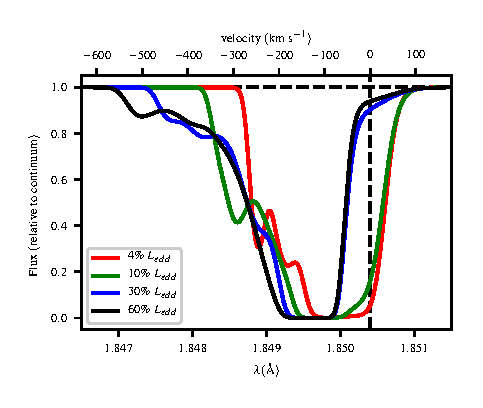
\includegraphics[width=\columnwidth]{figures/80_degrees_fe25.eps}
\caption{Simulated line profile for the Fe~\textsc{xxv} Lyman~$\rm{\alpha}$
transition at 1.85~{\AA}, as viewed from $i = 80\degree$ for a range
of luminosities.}
\label{figure:line25}
\end{figure}

There are two interesting observations to be made from this plot. Firstly, the maximum velocity seen in 
the line increases with luminosity. Secondly, there is a notable difference between the line two lower luminosity 
profiles and the higher pair. All lines exhibit some absorption at about $\rm{+100~kms^{-1}}$, due to thermal 
broadening of absorption from stationary or slow moving material. However for the 4 per cent and 10 per cent 
cases the feature is almost black at $\rm{0~kms^{-1}}$ indicating the presence of more slow moving material than 
in the 30 and 60 per cent cases. As discussed in Section \ref{Section:B83}, the two higher luminosity runs
are in the ``isothermal'' part of Figure \ref{figure:regions} and the gas in these cases would be expected to 
be more impulsively heated. Whist the gas does not reach the Compton temperature in either case, the 
shape of the lines does point to a faster heating process and a quicker acceleration. 


Another line commonly seen in XRB winds is the Lyman $\alpha$ resonance 
line of Fe~\textsc{xxvi} which is actually a doublet with components at
1.778~{\AA} and 1.783~{\AA}. The ray traced absorption profile for this 
feature is given as the thin lines in Figure \ref{figure:line26_smooth}. The absorption profile
as a function of velocity in each of the two lines is almost identical to that seen in the 
Fe \textsc{xxv} feature shown in Figure \ref{figure:line25} but these features
are slightly less
saturated and hence there is a range of EWs for the doublet, ranging from -8~eV for the 4\% $\rm{L_{Edd}}$
run to -16~eV for the 60\% luminosity. The run at the Eddington luminosity 
has an EW of almost 20eV, but this should be treated with caution because of the lack
of radiation driving in our simulation. If radiation driving is important as would be expected then one would expect
a significantly larger EW.

The current generation of X-ray spectrometers are unable to split this feature
into its components; for example the wavelength resolution of the \emph{Chandra}
HETG is 0.012\AA~ compared to the feature spacing of 0.005\AA.
 Therefore the feature is always observed as a single line. The heavy lines in Figure 
 \ref{figure:line26_smooth}
show the line pair smoothed by a Gaussian to reproduce the appearance of this line
through the \emph{Chandra} HETG. 


\begin{figure}
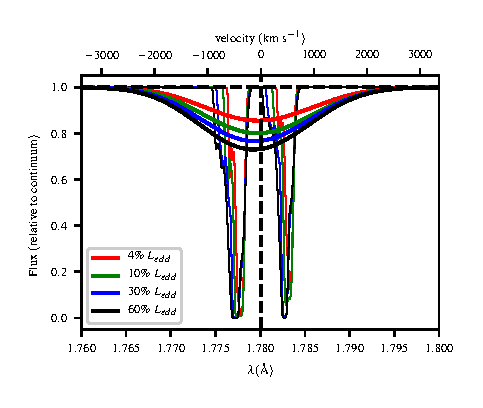
\includegraphics[width=\columnwidth]{figures/80_degrees_fe26_smooth.eps}
\caption{Simulated line profile for the Fe~\textsc{xxvi} Lyman~$\rm{\alpha}$
doublet, as viewed from $i = 80\degree$ for a range
of luminosities (thin lines) and also smoothed with a Gaussian to represent the appearance when
observed with the \emph{Chandra} HETG with a resolution of 0.012\AA~(thick lines)}
\label{figure:line26_smooth}
\end{figure}

The EW of lines observed in X-ray binary disk winds are mostly around 10-30eV 
\cite{2012MNRAS.422L..11P}, 
similar to the 
values we obtain here. The velocities are higher however, ranging between about 400-3000 $\rm{kms^{-1}}$
\cite{2016AN....337..368D}. It is possible that the including of continuum driving would accelerate the winds
to higher velocities. This would tend to increase the EW since the lines in our simulations are black in 
places, and this dense gas would be more distributed in velocity space. 


\subsection{Kinetic Luminosity}

Whilst the mass loss is of interest when considering how the wind could affect the 
accretion flow through the disk, it is also interesting to consider what (if any) effect the
wind could have on the surroundings. The kinetic energy carried by the wind is a
good measure of this, and so we calculate this via a simple summation around the outer
edge of the domain. 

\begin{figure}
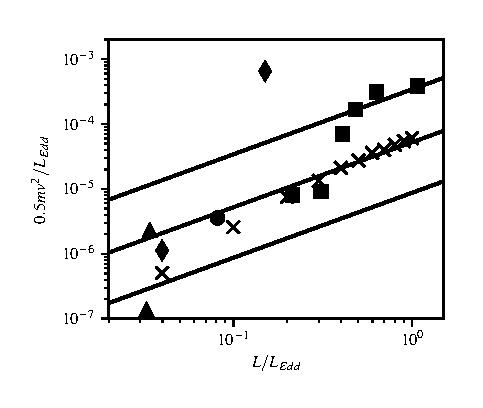
\includegraphics[width=\columnwidth]{figures/lum_vs_ke_ponti.eps}
\caption{Kinetic energy transported by the wind  as a function of source luminosity, both
normalised to the Eddington luminosity. Crosses are for this work, the other symbols represent
date from
\protect\cite{2016AN....337..512P}, the symbols code for different sources as in Figure \ref{figure:mdot_vs_lum}.
The diagonal lines show theoretical calculations of kinetic luminosity assuming a 0.1 per cent conversion
from luminosity to kinetic energy for disks with 1\degree, 6\degree~ and 40\degree~ total flare.}
\label{figure:ke_vs_lum}
\end{figure}

The results are plotted in Figure \ref{figure:ke_vs_lum} together with observed values from
\cite{2016AN....337..512P} for the same sources as plotted in Figure \ref{figure:mdot_vs_lum}. 
Taking into account the flare of the disk (which is 4\degree~ for the lowest luminosity rising to 6\degree for
the $\rm{L=L_{Edd}}$ run the efficiency of conversion from intercepted radiative luminosity into kinetic 
energy is about 0.1 per cent for our runs with $\rm{L \geq 0.2L_{Edd}}$. For the two lower luminosity runs,
the efficiency is lower, at 0.04 per cent for $\rm{0.04L_{Edd}}$ and 0.06 per cent for $\rm{0.1L_{Edd}}$.
Interestingly these are the two runs where the luminosity is below $\rm{L_{crit}}$.

The flare seen in our simulations is a function of the radiative transfer process as discussed earlier, and we 
do not include any underlying flare in the accretion disk. It has been shown that at high Eddington fractions,
accretion disks tend to puff up to larger scale heights \citep[][but also see \citealt{2016A&A...587A..13L}]{1988ApJ...332..646A,2005MNRAS.357..295O} and so we would
expect such a disk to intercept a greater fraction of the incoming radiation. This could explain the way in which 
the observed kinetic energy flux dramatically increases at luminosities greater than 30 per cent Eddington. The
diagonal lines show the relationship between radiative and kinetic luminosity for 1\degree,~6\degree and 40\degree~
total disk flare angles. We see that as expected our results tend to the 6\degree~ line, and if the efficiency is 
the same at all higher luminosities we would require a disk opening angle of 40\degree~ to explain the high 
luminosity results. It is possible that the efficiency could also increase when radiation driving is included.


\subsection{Effect of radiation driving}

As the luminosity increases, one should include the effects
of radiation pressure on the simulation. For such a relatively hard SED, 
the plasma above the disk will by largely ionized, and so electron
pressure would be the only radiation pressure one would expect. The 
effect can be though of as effectively a reduction in the inner radius
at which a wind is launched. \cite{2018MNRAS.473..838D} give this 
correction as
\begin{equation}
\overline{R}_{IC}\approx R_{IC}\left(1-\frac{L}{0.71L_{Edd}}\right)
\end{equation}
which means that the wind can be launched from all radii at a luminosity
of $0.71 L_{Edd}$. This in turn means that our mass loss rates will be a lower 
bound for luminosities approaching or exceeding this value. We can make a rough
estimate of the the effect on the mass-loss rate of including radiation driving by
noting that for the 60 per cent and 100 per cent Eddington runs, the mass-loss
rate per unit area is approximately proportional to $R^{-1.5}$. If all the radii
interior to where the wind current arises were to follow this relationship, then the 
mass-loss would increase by a factor of about 1.5. 
We might also 
expect somewhat higher velocities in the outflow, due to the additional force, which could also
increase the efficiency of conversion from radiative luminosity into kinetic luminosity as previously
mentioned. 
We are planning to include this effect in our next set of simulations.





\section{Summary }

Thermal driving is an attractive mechanism to explain the outflows observed in several 
X-ray binaries seen at high inclinations. We have previously demonstrated that 
the outflow seen in the soft-intermediate state of GRO J1655-40 could be plausibly 
modelled by a thermal wind, and here we extend that work to higher luminosities. We find

\begin{itemize}
\item{As the luminosity (and therefore accretion rate) increases, so does the mass-loss rate through the wind. 
The ratio between the two, $\dot{\rm{M}}_{\rm{wind}}/\dot{\rm{M}}_{\rm{acc}}$ or the wind efficiency,
tends to a constant value of around 2. This is in agreement with previous theoretical studies and 
also observations.}
\item{At the luminosity increases, the maximum blue shifted velocities seen in a simulated 
Fe \textsc{xxv} and Fe \textsc{xxvi} absorption lines increases. There is also less material at low 
velocities as the material is more impulsively heated.}
\item{The kinetic energy transported by the wind also increases with luminosity however; the efficiency of conversion from radiative luminosity to kinetic 
luminosity is about 0.1 per cent. Differences between our predicted kinetic energy and observations could be explained
by either a difference in efficiency (possibly due to continuum driving) or an increased underlying disk flare at high
luminosities.}

These simulations do not include the effects of radiation driving, which may become
important at higher luminosities. 



\end{itemize}

\section{acknowledgements}
Calculations in this work made use of the Iridis4 Supercomputer at the University of Southampton.
NH and CK  acknowledge support by the Science and Technology Facilities Council grant ST/M001326/1. 
KSL acknowledges the support of NASA for this work through grant NNG15PP48P to serve as a 
science adviser to the Astro-H project, JHM is supported by STFC grant ST/N000919/1 and SAS 
is supported by STFC through grant, ST/P000312/1. 



\bibliographystyle{mnras}
\bibliography{bibliography}()
\label{lastpage}

% Don't change these lines
\bsp	% typesetting comment

\end{document}

% End of mnras_template.tex
